%%%%%%%%%%%%%%%%%%%%%%%%%%%%%%%%%%%%%%%%%
% LaTeX Template
%%%%%%%%%%%%%%%%%%%%%%%%%%%%%%%%%%%%%%%%%

%----------------------------------------------------------------------------------------
%	PACKAGES AND DOCUMENT CONFIGURATIONS
%----------------------------------------------------------------------------------------

\documentclass[11pt,twoside,a4paper]{article}
\usepackage{geometry}

\usepackage{siunitx} % Provides the \SI{}{} and \si{} command for typesetting SI units
\usepackage{graphicx} % Required for the inclusion of images
\usepackage[square,sort,comma,numbers]{natbib}
\usepackage{amsmath} % Required for some math elements
\usepackage{lastpage} % know last page (used in fancy header)
\usepackage{fancyhdr} % Fancy Header
\usepackage[xindy, toc, numberedsection]{glossaries} % glossaries with xindy (recommended) for the indexing phase and show glossaries in TOC, and numberedsection to get a Setion number in the title
\usepackage{url} %The command is intended for email addresses, hypertext links, directories/paths, etc., which normally have no spaces, so by default the package ignores spaces in its argument.
\usepackage{minted} % it allows formatting and highlighting source code
% in addition, Pygments must be installed
% How to install on Windows:
% 1) install python (and add it to your PATH)
% 2) install pip (https://pip.pypa.io/en/stable/installing/)
% 3) install pygments (pip install Pygments)
% add pygments to your PATH, the command "pip show Pygments" shows where the lib is installed
% Of course, pdfLaTeX (or whatever engine/format you use) still has to be called with the -shell-escape option.
\usepackage{pgf}
\usepackage{booktabs}
\usepackage[dutch]{babel}
\usepackage[]{subfig}
\usepackage[]{textcmds} % voor quotes
\usepackage[]{listings}

\loadglsentries{glossaries.tex}
\makeglossaries % generate the glossary
% Any links in resulting glossary will not be "clickable" unless you load the glossaries package after the hyperref package.

\setlength\parindent{0pt} % Removes all indentation from paragraphs

\renewcommand{\labelenumi}{\alph{enumi}.} % Make numbering in the enumerate environment by letter rather than number (e.g. section 6)

\renewcommand{\arraystretch}{1.5} % Increasing the array stretch factor using \renewcommand{\arraystretch}{<factor>} where <factor> is a numeric value

%\usepackage{times} % Uncomment to use the Times New Roman font

%----------------------------------------------------------------------------------------
%	DOCUMENT INFORMATION
%----------------------------------------------------------------------------------------
\newcommand{\maintitle}{GRAYSCALE - EDGE DETECTION}
\newcommand{\course}{Labo Geavanceerde Computertechniek}
\newcommand{\coursenumber}{JLIZNM}
\newcommand{\class}{MELICTEES}

%%%%%%%%%%%%%%%%%%%%%%%%%%%%%% HEADER %%%%%%%%%%%%%%%%%%%%%%%%%%%%%%
\pagestyle{fancy}
\fancyhf{}
\fancyhead[LE,RO]{\course}
\fancyhead[RE,LO]{\maintitle}
% if working with chapters
% \fancyfoot[CE,CO]{\leftmark}
\fancyfoot[LE,RO]{\thepage\ of \pageref{LastPage}}
%%%%%%%%%%%%%%%%%%%%%%%%%%%%%% HEADER %%%%%%%%%%%%%%%%%%%%%%%%%%%%%%


%%------------------------------ TITLE PAGE -----------------------------
\title{\maintitle \\ \course \\{\small\ (\coursenumber)}} % Title

\author{Jona \textsc{Cappelle} \& \textsc{Jonas Bolle}} % Author name

\date{\today} % Date for the report

\begin{document}\sloppy % sloppy is used to enforce that lines are in hbox
\newgeometry{hmarginratio=1:1}    %% make layout symmetric
\pagenumbering{gobble}% Remove page numbers (and reset to 1)
\begin{titlepage}
\maketitle % Insert the title, author and date

\vfill
\begin{center}

\includegraphics[width=0.13\textwidth]{logo_kuleuven.png} %
\end{center}
%each \vfill will expand vertically the same amount until the entire page is filled
\vfill
\vfill
\vfill

\begin{center}
\begin{tabular}{l r}
Sessie Datum: & 4 Mei, 2020 \\ % Date the experiment was performed
\\
Partners: &  Jona Cappelle\\ % Partner names
&  Jonas Bolle\\
Klas: & \class \\
\\
Begeleider: &  Stijn Crul% Instructor/supervisor
\end{tabular}
\end{center}
\vfill
\vfill
\end{titlepage}
\clearpage
\newpage\null\thispagestyle{empty}\newpage % blank page after title page

%%------------------------------ TITLE PAGE -----------------------------


\restoregeometry%              %% restore the layout
\pagenumbering{arabic}% Arabic page numbers (and reset to 1)

\tableofcontents
\listoffigures
\listoftables
\listoflistings
\clearpage

%----------------------------------------------------------------------------------------
%	INLEIDING
%----------------------------------------------------------------------------------------
\section{Inleiding}

In dit labo van geavanceerde computertechniek gaan we een grayscale van een afbeelding maken en edge detection toepassen.

Een grayscale operatie zet alle kleurenwaarden om naar zwart-wit waarden met een equivalente luminantie. Een edge detection operatie detecteert grote verschillen tussen naburige pixels.

%----------------------------------------------------------------------------------------
%	PROBLEEMSTELLING
%----------------------------------------------------------------------------------------
% \section{Probleemstelling}


% welke uitdagingen
% wat wordt er onderzocht

%----------------------------------------------------------------------------------------
%	OPLOSSING
%----------------------------------------------------------------------------------------

%----------------------------------------------------------------------------------------
%	ANALYSE PERFORMANTIE
%----------------------------------------------------------------------------------------
\section{Probleemstelling en analyse performantie}

%----------------------------------------------------------------------------------------
\subsection{Grayscale}
%----------------------------------------------------------------------------------------

De bedoeling van het eerste deel van het labo is het omzetten van een kleurenafbeelding in een grayscale afbeelding. Het resultaat hiervan is terug te vinden in figuur \ref{fig:grayscale}. Bij de grayscale zijn er verschillende mogelijkheden om deze te implementeren. Men kan het gemiddelde nemen van de RGB waarden en dit gemiddelde toekennen aan elke R, G en B waarde. Er kan ook gewerkt worden met verschillende verhoudingen voor RGB waarden. In dit labo hebben we voor deze eerste optie gekozen.

De ingelezen afbeelding zetten we met \q{lodepng} om naar een \'e\'endimensionale array met structuur zoals weergegeven in figuur \ref{fig:1}.



    \begin{figure}[h!]
        \centering

    \begin{tabular}{|c|c|c|c|}
    \hline
    image{[}i{]} & image{[}i+1{]} & image{[}i+2{]} & image{[}i+3{]} \\ \hline
    Red          & Green          & Blue           & Alpha          \\ \hline
    \end{tabular}

        \caption{Opbouw PNG afbeelding}
        \label{fig:1}
    \end{figure}

    Hier moeten we er rekening mee houden dat het \q{alpha} kanaal, dat de opacity bepaalt, altijd de waarde 255 moet hebben om de afbeelding niet doorzichtig te maken.

    De code van grayscale is terug te vinden in deel \ref{code_grayscale} op pagina \pageref{code_grayscale} en volgende.


\begin{figure}[h!]
    \centering
    \subfloat[Input]{
\includegraphics[width=0.5\columnwidth]{input.png}}
    \hfill
    \subfloat[Output]{
\includegraphics[width=0.5\columnwidth]{output_grayscale.png}}
    \caption{Resultaat grayscale}
    \label{fig:grayscale}
\end{figure}


\subsubsection{Tijd op GPU}

We meten de uitvoertijd op de GPU bij verschillende blocksizes. Hier werd het kopi\"eren van de data van en naar de GPU niet mee in rekening gebracht. De laagste tijden worden bekomen bij blocksizes met veelvouden van 32. Een grafiek hiervan is terug te vinden in figuur \ref{fig:meting_grayscale_gpu}.

De tijd die het duurt om de grayscale uit te voeren is:
\begin{align*}
    &t_{GPU} = \SI{304}{\micro s}
\end{align*}


\begin{figure}[h!]
    \centering
    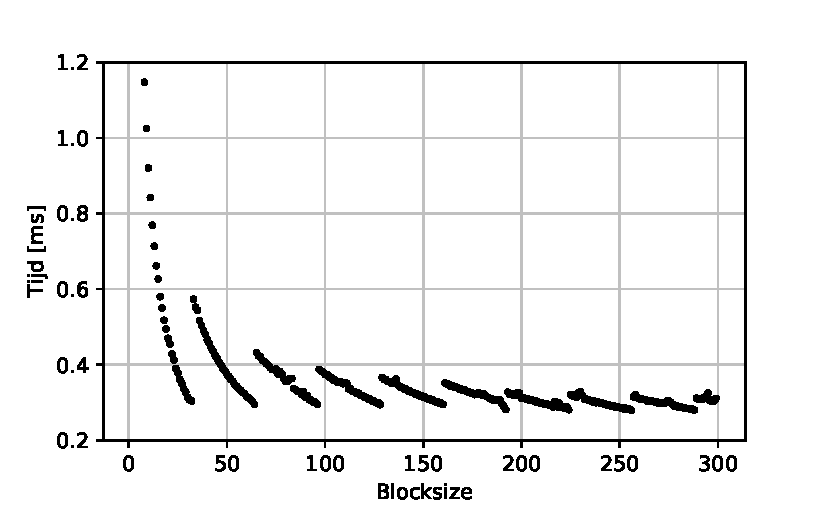
\includegraphics[]{gpu_grayscale.pdf}
    \caption{Meting tijd op GPU bij verschillende blocksizes}
    \label{fig:meting_grayscale_gpu}
\end{figure}


\subsubsection{Tijd op CPU}

Wanneer we een gray scale implementatie op de CPU schrijven, duurt het veel langer om deze uit te voeren namelijk:
\begin{align*}
    &t_{CPU} = \SI{656}{\micro s}
\end{align*}

Dit is meer dan dubbel zo lang dan de uitvoering op de GPU (zonder mee kopi\"eren van de data). Uit vorig labo konden we al besluiten dat het langer zal duren met het mee kopi\"eren van de data maar dat bij een groot aantal fotos die omgezet moeten worden de GPU met zijn parallelisatie toch veel sneller zal zijn. Om deze reden werd deze meting hier niet opnieuw gedaan.

%----------------------------------------------------------------------------------------
\subsection{Edge detection}
%----------------------------------------------------------------------------------------

In het tweede deel van het labo gaan we edge detection toepassen op een afbeelding. Het resultaat van deze operatie is terug te vinden in figuur \ref{fig:edge_dection}. Edge detection is een mooi vervolg op grayscale, daar we de grayscale ook nodig hebben om aan edge detection te doen. Voor de edge detection werd gewerkt met de gekende sobel filter. Het werkt op basis van een 3x3 matrix vermenigvuldiging met elke pixel van het beeld. Wanneer er veel verschil is naburige waarden van pixels, zal deze bewerking ofwel een zeer groot, of een zeer klein resultaat opleveren. We maken gebruik van twee 3x3 matrices, \'e\'en voor de veranderingen in de x-richting te detecteren ($G_x$) en \'e\'en voor de veranderingen in de y-richting te detecteren ($G_y$). Om deze waarden samen te voegen ($G$) en negatieve getallen te vermijden, wordt hier ook de wortel van de kwadraten van beide x en y resultaten genomen.

\begin{figure}[H]
    \centering
    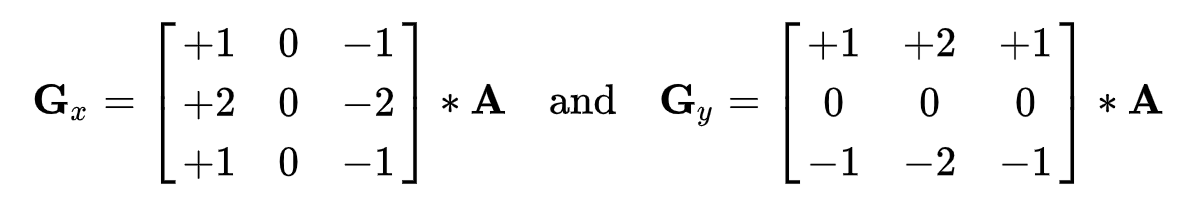
\includegraphics[scale=0.3]{1.png}
    \caption*{}
    \label{fig:formule1}
\end{figure}

\begin{figure}[H]
    \centering
    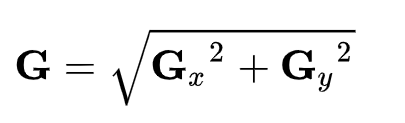
\includegraphics[scale=0.3]{2.png}
    \caption*{\cite{sobel}}
    \label{fig:formule2}
\end{figure}


\begin{figure}[h!]
    \centering
    \subfloat[Input]{
\includegraphics[width=0.5\columnwidth]{input.png}}
    \hfill
    \subfloat[Output]{
\includegraphics[width=0.5\columnwidth]{output_edge_detection.png}}
    \caption{Resultaat edge detection GPU}
    \label{fig:edge_dection}
\end{figure}



De code van edge detection is terug te vinden in deel \ref{code_edge_detection} op pagina \pageref{code_edge_detection} en volgende.


\subsubsection{Tijd op GPU}

Als we de edge detectie op de GPU uitvoeren, duurt het:
\begin{align*}
    &t_{GPU} = \SI{336}{\micro s}
\end{align*}

Hierbij werd rekening gehouden met het optimaal aantal threads per block een veelvoud te kiezen van 32. Zie listing \ref{listing1}. Er werd gekozen voor een Blocksize van 64 op 16 = 1024. nBlocks volgt hieruit: 64 (4 op 16). Door hier in 2D de threads te organiseren, laat dit ons toe de edge detection op de gpu intu\"itiever te coderen. De threads die naast en onder elkaar staan, zullen ook de waarden van de pixels berekenen die naast en onder elkaar staan.

\begin{lstlisting}[language=C, caption=Keuze Blocksize en nBlock, frame=single]
	// Choose Blocksize & nBlock in 2D
	dim3 BLOCKSIZE(64,16);
	dim3 nBlocks(ceil(width/64),ceil(height/16));
\end{lstlisting}\label{listing1}


\subsubsection{Tijd op CPU}
%TODO
Als we de edge detectie op de CPU uitvoeren, duurt het:
\begin{align*}
    &t_{CPU} = \SI{3496}{\micro s}
\end{align*}



\begin{figure}[h!]
    \centering
    \subfloat[Input]{
\includegraphics[width=0.5\columnwidth]{input.png}}
    \hfill
    \subfloat[Output]{
\includegraphics[width=0.5\columnwidth]{outputcpu.png}}
    \caption{Resultaat edge detection CPU}
    \label{fig:edge_dection_cpu}
\end{figure}

Dit is 10 keer langer dan de bewerking op de GPU! Hoe intensiever de taken worden, hoe groter de tijdswinst als we te werk gaan met een GPU.

Het resultaat van de edge detection op de CPU is terug te vinden in figuur \ref{fig:edge_dection_cpu}.


%----------------------------------------------------------------------------------------
%	BESLUIT
%----------------------------------------------------------------------------------------
\clearpage
\section{Besluit}
% waarom goed / niet goed

% Please add the following required packages to your document preamble:
% \usepackage{booktabs}
% \usepackage{graphicx}
\begin{table}[h!]
    \centering
    \begin{tabular}{@{}lll@{}}
    \toprule
    Grayscale      &             &  \\ \midrule
                   & Tijd op GPU &  \SI{304}{\micro s}\\
                   & Tijd op CPU &  \SI{656}{\micro s}\\
    \toprule
    Edge detection &             &  \\ \midrule
                   & Tijd op GPU &  \SI{336}{\micro s}\\
                   & Tijd op CPU &  \SI{3496}{\micro s}\\ \bottomrule %TODO
    \end{tabular}%
    \caption{Samenvattende tabel tijden CPU en GPU}
    \label{tab:samenvattende_tabel}
    \end{table}

Uit tabel \ref{tab:samenvattende_tabel} kunnen we besluiten dat het uitvoeren van bewerkingen op de GPU veel sneller kan gebeuren dan op een CPU. 

Ook hier zien we terugkomen dat 32 threads per block optimaal is voor performantie. Dit komt aangezien CUDA GPU's kernels runnen die blokken van threads gebruiken met een veelvoud van 32. Indien de gebruiker ook dit veelvoud van 32 hanteert, zal er zoveel mogelijk parallelisatie optreden. Wanneer niet voor dit veelvoud gekozen wordt, zullen enkele threads niet gebruikt worden en zal het programma bijgevolg trager uitgevoerd worden.

Een andere conclusie die we kunnen maken is dat de edge detection langer duurt dan de grayscale. Bij de grayscale wordt enkel het gemiddelde van de pixels genomen: twee optellingen en \'e\'en vermenigvuldiging. Bij de edge detection wordt er vermenigvuldigd met twee maal een 3x3 matrix, wat meer tijd vergt (meer vermenigvuldigingen en optellingen).

Conclusie: Bij zeer kleine workloads heeft het kopi\"eren van data van en naar de GPU een grote invloed op de uitvoeringstijd. Bij grotere parallele workloads is het veel sneller om een GPU te gebruiken dan een CPU. Dit kunnen we ook zien aan de speedup factor van de grayscale functie en de egde detection functie: de GPU voert de grayscale functie 2x sneller uit dan de CPU, bij de egde detection is dit x10! 

%----------------------------------------------------------------------------------------
%----------------------------------------------------------------------------------------

\newpage
\appendix

%----------------------------------------------------------------------------------------
%----------------------------------------------------------------------------------------

% \newpage
\section{CODE GRAYSCALE}\label{code_grayscale}
\inputminted[linenos=true, breaklines=true]{cuda}{main.cu}
\clearpage
\section{CODE EDGE DETECTION}\label{code_edge_detection}
\inputminted[linenos=true, breaklines=true]{cuda}{edge.cu}

%----------------------------------------------------------------------------------------
%	BIBLIOGRAPHY
%----------------------------------------------------------------------------------------
\clearpage
\bibliographystyle{IEEEtranN}
\bibliography{bib}

%----------------------------------------------------------------------------------------

\end{document}
